%%**************************************************************
%% Vorlage fuer Bachelorarbeiten (o.ä.) der DHBW
%%
%% Autor: Tobias Dreher, Yves Fischer
%% Datum: 06.07.2011
%%**************************************************************

\newcommand{\pdftitel}{PDF Title of the document}
\newcommand{\autor}{Max Mustermann}
\newcommand{\arbeit}{Bachelor thesis}

%
% Nahezu alle Einstellungen koennen hier getaetigt werden
%

\documentclass[%
	pdftex,
	oneside,        % Einseitiger Druck.
	12pt,           % Schriftgroesse
	parskip=half,   % Halbe Zeile Abstand zwischen Absätzen.
	headsepline,    % Linie nach Kopfzeile.
	footsepline,    % Linie vor Fusszeile.
	abstracton,     % Abstract Überschriften
	english,        % Translator
]{scrreprt}

%Seitengroesse
\usepackage{fullpage}

%Zeilenumbruch und mehr
\usepackage[activate]{microtype}

% Zeichencodierung
\usepackage[utf8]{inputenc}
\usepackage[T1]{fontenc}

% Zeilenabstand
\usepackage[onehalfspacing]{setspace}

% Index-Erstellung
\usepackage{makeidx}

% Lokalisierung (englische Sprache)
\usepackage[english]{babel}

% Anführungszeichen 
\usepackage[babel,german=quotes]{csquotes}
%\usepackage[style=swiss]{csquotes}


% Spezielle Tabellenform fuer Deckblatt
\usepackage{longtable}
\setlength{\tabcolsep}{10pt} %Abstand zwischen Spalten
\renewcommand{\arraystretch}{1.5} %Zeilenabstand

% Grafiken
\usepackage{graphicx}

% Mathematische Textsaetze
%\usepackage{amsmath}
%\usepackage{amssymb}

% Pakete um Textteile drehen zu können, oder eine Seite Querformat anzeigen kann.
%\usepackage{rotating}
%\usepackage{lscape}

% Farben
\usepackage{color}
\definecolor{LinkColor}{rgb}{0,0,0.2}
\definecolor{ListingBackground}{rgb}{0.92,0.92,0.92}

% PDF Einstellungen
\usepackage[%
	pdftitle={\pdftitel},
	pdfauthor={\autor},
	pdfsubject={\arbeit},
	pdfcreator={pdflatex, LaTeX with KOMA-Script},
	pdfpagemode=UseOutlines, % Beim Oeffnen Inhaltsverzeichnis anzeigen
	pdfdisplaydoctitle=true, % Dokumenttitel statt Dateiname anzeigen.
	pdflang=eng % Sprache des Dokuments.
]{hyperref}

% (Farb-)einstellungen für die Links im PDF
\hypersetup{%
	colorlinks=false, % Aktivieren von farbigen Links im Dokument
	linkcolor=LinkColor, % Farbe festlegen
	citecolor=LinkColor,
	filecolor=LinkColor,
	menucolor=LinkColor,
	urlcolor=LinkColor,
	bookmarksnumbered=true % Überschriftsnummerierung im PDF Inhalt anzeigen.
}

% Verschiedene Schriftarten
%\usepackage{goudysans}
%\usepackage{lmodern}
%\usepackage{libertine}
\usepackage{palatino} 

% Hurenkinder und Schusterjungen verhindern
% http://projekte.dante.de/DanteFAQ/Silbentrennung
\clubpenalty=10000
\widowpenalty=10000
\displaywidowpenalty=10000

% Quellcode
\usepackage{listings}
\lstloadlanguages{Java}
\lstset{%
	language=PHP,            % Sprache des Quellcodes
	%numbers=left,           % Zeilennummern links
	stepnumber=1,            % Jede Zeile nummerieren.
	numbersep=5pt,           % 5pt Abstand zum Quellcode
	numberstyle=\tiny,       % Zeichengrösse 'tiny' für die Nummern.
	breaklines=true,         % Zeilen umbrechen wenn notwendig.
	breakautoindent=true,    % Nach dem Zeilenumbruch Zeile einrücken.
	postbreak=\space,        % Bei Leerzeichen umbrechen.
	tabsize=2,               % Tabulatorgrösse 2
	basicstyle=\ttfamily\footnotesize, % Nichtproportionale Schrift, klein für den Quellcode
	showspaces=false,        % Leerzeichen nicht anzeigen.
	showstringspaces=false,  % Leerzeichen auch in Strings ('') nicht anzeigen.
	extendedchars=true,      % Alle Zeichen vom Latin1 Zeichensatz anzeigen.
	captionpos=b,            % sets the caption-position to bottom
	backgroundcolor=\color{ListingBackground} % Hintergrundfarbe des Quellcodes setzen.
}

% Glossar
\usepackage[
	nonumberlist, %keine Seitenzahlen anzeigen
	acronym,      %ein Abkürzungsverzeichnis erstellen
	%section,     %im Inhaltsverzeichnis auf section-Ebene erscheinen
	toc,          %Einträge im Inhaltsverzeichnis
]{glossaries}

% Fussnoten
\usepackage[perpage, hang, multiple, stable]{footmisc}

% Titel, Autor und Datum
\title{\titel}
\author{\autor}
\date{\datum}


% Ab jetzt können auch Umlaute verwendet werden
\newcommand{\titel}{Usually the title of a Bachelor thesis has a length of two lines}
\newcommand{\matrikelnr}{1234567}
\newcommand{\kurs}{ABC2008DE}
\newcommand{\datumAbgabe}{August 2011}
\newcommand{\firma}{Firma GmbH}
\newcommand{\firmenort}{Firmenort}
\newcommand{\abgabeort}{Abgabeort}
\newcommand{\abschluss}{Bachelor of Arts}
\newcommand{\studiengang}{Vorderasiatische Archäologie}
\newcommand{\dhbw}{Stuttgart Campus Horb}
\newcommand{\betreuer}{Dipl.-Ing. (FH) Peter Pan}
\newcommand{\gutachter}{Dr. Silvana Koch-Mehrin}
\newcommand{\zeitraum}{12 Weeks}

\makeglossaries
%
% vorher in Konsole folgendes aufrufen: 
%	makeglossaries makeglossaries dokumentation.acn && makeglossaries dokumentation.glo
%

%
% Abkürzungen --> referenz, name, beschreibung
% Aufruf mit \gls{...} oder Kurzform mit \acrshort{...}
%

\newacronym{DHBW}{DHBW}{Duale Hochschule Baden Württemberg}
\newacronym{I2CBus}{I\textsuperscript{2}C-Bus}{Inter-Integrated-Circuit-Bus}

%
% Glossareintraege --> referenz, name, beschreibung
% Aufruf mit \gls{...}
%
\newglossaryentry{Glossareintrag}{name={Glossareintrag},plural={Glossareinträge},description={Ein Glossar beschreibt verschiedenste Dinge in kurzen Worten}}


\begin{document}

	% Deckblatt
	\begin{spacing}{1}
		\begin{titlepage}
	\begin{longtable}{p{.55\textwidth} p{.85\textwidth}}
	  {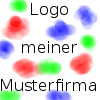
\includegraphics[height=2.6cm]{images/logo.png}} & 
	  {
\includegraphics[height=2.6cm]{images/dhbw.png}}
	\end{longtable}
	\enlargethispage{20mm}
	\begin{center}
	  \vspace*{12mm}	{\LARGE\textbf \titel }\\
	  \vspace*{12mm}	{\large\textbf \arbeit}\\
	  \vspace*{12mm}	for the\\
	  \vspace*{3mm} 	{\textbf \abschluss}\\
	  \vspace*{12mm}	from the Course of Studies \studiengang\\
	  \vspace*{3mm} 	at the Cooperative State University Baden-Württemberg \dhbw\\
	  \vspace*{12mm}	by\\
	  \vspace*{3mm} 	{\large\textbf \autor}\\
	  \vspace*{12mm}	\datumAbgabe\\
	\end{center}
	\vfill
	\begin{spacing}{1.2}
	\begin{tabbing}
		mmmmmmmmmmmmmmmmmmmmmmm     \= \kill
		\textbf{Time of Project}  \>  \zeitraum\\
		\textbf{Student ID, Course}  \>  \matrikelnr, \kurs\\
		\textbf{Company}      \>  \firma, \firmenort\\
		\textbf{Supervisor in the Company}              \>  \betreuer\\
		\textbf{Reviewer}             \>  \gutachter
	\end{tabbing}
	\end{spacing}
\end{titlepage}

	\end{spacing}
	\newpage
	
	\pagenumbering{Roman}
	
	% Sperrvermerk
	%!TEX root = ../dokumentation.tex

\thispagestyle{empty}
% Sperrvermerk direkt hinter Titelseite
\section*{Confidentiality Statement}

\vspace*{2em}

%http://www.ib.dhbw-mannheim.de/fileadmin/ms/bwl-ib/Downloads_alt/Leitfaden_31.05.pdf

  The {\arbeit} on hand 
  \begin{center}{\itshape{} \titel{}\/}\end{center} 
   contains internal resp.\ confidential data of {\firma}. It is intended solely for inspection by the assigned examiner, the head of the {\studiengang} department and, if necessary, the Audit Committee at the Cooperative State University Baden-Württemberg {\dhbw}. It is strictly forbidden
    \begin{itemize}
    \item to distribute the content of this paper (including data, figures, tables, charts etc.) as a whole or in extracts,
    \item to make copies or transcripts of this paper or of parts of it,
    \item to display this paper or make it available in digital, electronic or virtual form.
    \end{itemize}
  Exceptional cases may be considered through permission granted in written form by the author and {\firma}.

\vspace{3em}

\abgabeort, \datumAbgabe
\vspace{4em}

\rule{6cm}{0.4pt}\\
\autor

	\newpage
	
	% Erklärung
	\thispagestyle{empty}

\section*{Author's declaration}
% Seite 8  http://studium.ba-bw.de/fileadmin/media/allgemein/bestimmungen/btechnik/richtlinien/Richtlinien_Praxismodule_Studien_und_Bachelorarbeiten_2011.pdf
% http://www.ib.dhbw-mannheim.de/fileadmin/ms/bwl-ib/Downloads_alt/Leitfaden_31.05.pdf (S. 52)
\vspace*{2em}
Hereby I solemnly declare:
\begin{enumerate}
\item that this {\arbeit}, titled {\itshape \titel } is entirely the product of my own scholarly work, unless otherwise indicated in the text or references, or acknowledged below;
\item I have indicated the thoughts adopted directly or indirectly from other sources at the appropriate places within the document;
\item this {\arbeit} has not been submitted either in whole or part, for a degree at this or any other university or institution;
\item I have not published this {\arbeit} in the past; 
\item the printed version is equivalent to the submitted electronic one.
\end{enumerate}
I am aware that a dishonest declaration will entail legal consequences.
\vspace{3em}

\abgabeort, \datumAbgabe
\vspace{4em}

\rule{6cm}{0.4pt}\\
\autor



	\newpage

	% Abstract
	\pagestyle{empty}

\renewcommand{\abstractname}{Zusammenfassung}
\begin{abstract}
Ein Abstract ist eine prägnante Inhaltsangabe, ein Abriss ohne
Interpretation und Wertung einer wissenschaftlichen Arbeit. In DIN
1426 wird das (oder auch der) Abstract als Kurzreferat zur
Inhaltsangabe beschrieben.

\begin{description}
\item[Objektivität] soll sich jeder persönlichen Wertung enthalten
\item[Kürze] soll so kurz wie möglich sein
\item[Genauigkeit] soll genau die Inhalte und die Meinung der Originalarbeit wiedergeben
\end{description}

Üblicherweise müssen wissenschaftliche Artikel einen Abstract
enthalten, typischerweise von 100-150 Wörtern, ohne Bilder und
Literaturzitate und in einem Absatz.

Quelle \url{http://de.wikipedia.org/wiki/Abstract} Abgerufen 07.07.2011
\end{abstract}


\renewcommand{\abstractname}{Summary}
\begin{abstract}
An abstract is a brief summary of a research article, thesis, review,
conference proceeding or any in-depth analysis of a particular subject
or discipline, and is often used to help the reader quickly ascertain
the paper's purpose. When used, an abstract always appears at the
beginning of a manuscript, acting as the point-of-entry for any given
scientific paper or patent application. Abstracting and indexing
services for various academic disciplines are aimed at compiling a
body of literature for that particular subject.

The terms précis or synopsis are used in some publications to refer to
the same thing that other publications might call an "abstract". In
management reports, an executive summary usually contains more
information (and often more sensitive information) than the abstract
does.

Quelle: \url{http://en.wikipedia.org/wiki/Abstract_(summary)}

\end{abstract}

	\newpage

	\pagestyle{plain}		% nur Seitenzahlen im Fuß

	% Verzeichnisse

	\RedeclareSectionCommand[beforeskip=20pt]{chapter}	% stellt Abstand vor Kapitelüberschriften ein
%	\titlespacing*{\chapter}{0pt}{-50pt}{40pt} % this removes "before" spacing (the second length argument)
%	\renewcommand*\chapterheadstartvskip{\vspace*{-\topskip}} % this removes spacing before chapter titles

	% Inhaltsverzeichnis
	\begin{spacing}{1.1}
		\setcounter{tocdepth}{3}
		\tableofcontents
	\end{spacing}
	\newpage

	% Abkürzungsverzeichnis
	% vorher in Konsole folgendes aufrufen: 
	%	makeglossaries makeglossaries dokumentation.acn && makeglossaries dokumentation.glo
	\cleardoublepage
	\phantomsection \label{listofacs}
	\addcontentsline{toc}{chapter}{Abbreviations}
	%!TEX root = ../dokumentation.tex

\chapter*{Abbreviations}
%nur verwendete Akronyme werden letztlich im Abkürzungsverzeichnis des Dokuments angezeigt
%Verwendung: 
%		\ac{Abk.}   --> fügt die Abkürzung ein, beim ersten Aufruf wird zusätzlich automatisch die ausgeschriebene Version davor eingefügt bzw. in einer Fußnote (hierfür muss in header.tex \usepackage[printonlyused,footnote]{acronym} stehen) dargestellt
%		\acs{Abk.}   -->  fügt die Abkürzung ein
%		\acf{Abk.}   --> fügt die Abkürzung UND die Erklärung ein
%		\acl{Abk.}   --> fügt nur die Erklärung ein
%		\acp{Abk.}  --> gibt Plural aus (angefügtes 's'); das zusätzliche 'p' funktioniert auch bei obigen Befehlen
%	siehe auch: http://golatex.de/wiki/%5Cacronym
%
\begin{acronym}[YTMMM]
\setlength{\itemsep}{-\parsep}


\acro{AGPL}{Affero GNU General Public License}
\acro{AODV}{Ad-hoc On-Demand Distance Vector}
\acro{API}{Application Programming Interface}
\acro{DSR}{Dynamic Source Routing}
\acro{HTML}{HyperText Markup Language}
\acro{IEEE}{Institute of Electrical and Electronics Engineers}
\acro{LLC}{Logical Link Control }
\acro{MAC}{Medium Access Control}
\acro{MANET}{Mobile wireless Ad-hoc NETwork}
\acro{PHY}{Physical Layer}
\acro{QoS}{Quality of Service}
\acro{SPIN}{Sensor Protocol for Information via Negotiation}
\acro{WPAN}{Wireless Personal Area Network}
\acro{WMN}{Wireless Mesh Network}
\acro{WSN}{Wireless Sensor Network}
\acro{WYSIWYG}{What You See Is What You Get}
\end{acronym}

	\printglossary[type=\acronymtype]		% altes Abkürzungsverzeichnis

	% Abbildungsverzeichnis
	\cleardoublepage
	\listoffigures

	%Tabellenverzeichnis
	\cleardoublepage
	\listoftables

	% Quellcodeverzeichnis
	\cleardoublepage
	\lstlistoflistings
	\cleardoublepage

	\pagenumbering{arabic}
	\pagestyle{headings}		% Kolumnentitel im Kopf, Seitenzahlen im Fuß

	% Inhalt
	\foreach \i in {01,02,03,...,99} {%
		\edef\FileName{content/\i kapitel}%
			\IfFileExists{\FileName}{%
				\input{\FileName}
			}
			{%
				%file does not exist
			}
	}


	% Literaturverzeichnis
	\cleardoublepage
	\printbibliography
%	\phantomsection \label{listoflit}
%	\addcontentsline{toc}{chapter}{Bibliography}
	\begin{thebibliography}{---}

\bibitem[HAM10]{bib:ix042010}
  \textsc{Michael Hamm}: 
  \textbf{Der Erbe wächst - Freier Schwachstellen-Scanner OpenVAS 3.0}.
  iX Magazin, Ausgabe 4/2010, S. 81 ff., Heise Zeitschriften Verlag

\bibitem[NEU11]{bib:metasploitBuch}
  \textsc{Frank Neugebauer}: 
  \textbf{Penetration Testing mit Metasploit}.
  1. Auflage, 2011, dpunkt.verlag GmbH

\end{thebibliography}

		% altes Literaturverzeichnis

	% Glossar
	\printglossary[style=altlist,title=Glossary]
	
\end{document}
